% TODO

\chapter{Evaluation}
\label{chap:evaluation}
Throughout this thesis, we have designed, implemented, and deployed a \ac{SaaS} platform with a multi-tenant architecture aiming to fundamentally transform how eCommerce businesses interact with shipping carriers.
This platform covers the need for business to manage the specifics associated with each shipping carrier by automating the communication process and hiding all unnecessary details.
The platform's capabilities extend beyond mere data communication within expedition logistics; seeking into marketing corners with a tendency to present another possible marketing channel within post-purchase communication to enhance customer engagement.
Key features include an automated mechanism for customer email notifications triggered by changes in parcel statuses based on shipping carriers and tracking page.
Both are designed to serve as a post-purchase marketing channel with a seller's branding.
Allowing businesses to maintain continuous engagement with their customers while reinforcing brand identity.

This chapter delves into the evaluation of the platform, assessing its operational efficacy and integration within a real-world business environment.
The platform was integrated into a \textit{company} that handles more than 100 parcels per day, providing a robust testing ground for all the implemented features.
Integration was carried out on 14 March 2024.
This evaluation focuses on several critical areas:
\begin{itemize}
    \item The integration process with SAP Business One.
    \item Connecting with shipping carriers.
    \item Difficulty of training staff and problems that occurred during operation.
    \item The operational performance of the platform.
\end{itemize}
achieving the final goal of the project \hyperref[subsec:project-goals]{\textbf{G5}}.
By analysing these elements, we aim to validate the platform's design objectives and its potential to streamline logistics operations.


\section{Evaluation environments}
\label{sec:environments}
% local, staging, production
To ensure a comprehensive evaluation of the platform, the development and testing processes were conducted across three distinct environments: Local, Staging, and Production. 
Each environment played a specific role in the development life cycle, enabling incremental validation of features, performance testing, and secure deployment.


\subsection{Local development environment}
\label{subsec:local}
% serverless-offline
% docker database
The local environment primarily serves as the initial testing ground for development.
In this environment, we can quickly implement and test new features without the risk of affecting the live system. 
Leveraged Docker to run isolated instances of databases identical in structure to the production environment. 
This setup helped ensure that all database interactions were fully tested under controlled conditions, minimising irregularities between local and production behaviour.
In order to invoke functions and mimic server responses without connecting to the actual cloud service, the \gls{serverless-offline} plugin is used to simulate AWS Lambda and API Gateway locally. 

\subsection{Staging environment}
\label{subsec:staging}
% on the AWS
The staging environment mimics the production environment as closely as possible and served as the final step before full-scale deployment. 
It is hosted on AWS to simulate real world conditions using the same \ac{IaC} tools as in production, ensuring that all configurations were replicated.
This includes using \gls{aws-cloudformation} for resource orchestration and \gls{aws-lambda} to run backend services.
The staging environment is publicly accessible on a \texttt{staging} subdomain serving all services such as the dashboard, tracking page, and backend.

\subsection{Production environment}
\label{subsec:production}
% on the AWS
The production environment is where the platform fully operates and is accessible to the end users.
The platform is automatically deployed into the production environment always after successful deployment to the staging utilising close configurations.

By maintaining these distinct environments, we are able to systematically deploy updates, ensuring that each feature got tested before being released to the public. 
This structured approach not only minimises disruptions to live services, but also ensures that end users received a reliable and secure product.

\section{Production evaluation areas}
\label{ref:production-evalution-areas}
This section outlines the evaluation of the platform after its integration into a live business environment. 
The assessment focuses on four critical areas: integration with SAP Business One, connectivity with shipping carriers, training and operational challenges faced by staff, and the overall operational performance and business impact of the platform.
The first step was to create a user account and set up a project.
In this project, all operators were invited, the public API key was generated, as well as the setup of the so-called shipper address which serves as a return address for project shipments.

\subsection{Integration with SAP Business One}
\label{subsec:integration-with-sap}
Exchanging data with SAP Business One was a key element in the integration of the platform.
It required periodic exports of data from SAP to the platform and updates back into SAP with tracking numbers, the latest status, and delivery confirmation flags. 
To accomplish this, we used the SAP Service Layer Proxy and Data Sender, as detailed in Chapter \ref{chap:integrating-sap-b1}.
Storing data in the status of the parcel \texttt{metadata} retrieved from the PPL shipping carrier, such as invoice numbers, shipment costs, tolls and fuel taxes, proved beneficial. 
These data facilitated and accelerated monthly, mostly manual, shipping invoice processing tasks where the data provided on the invoice need to be checked and validated.
The integration process comprised three main phases:
Integration works with three phases of data exchange:
\begin{enumerate}
    \item \textbf{Exporting New Shipments:} In this initial phase, all packaged shipments are exported to the platform. This process runs every five minutes during operator working hours and picks shipments marked by the operator in the SAP Business One.
    \item \textbf{Updating New Shipments in SAP:} This phase updates all packed orders that have been exported to the platform and successfully dispatched to the carrier with a new status \texttt{DATA\_SENT} and the tracking number.
    \item \textbf{Periodic Status Update:} Each night, the Data Sender queries all previously shipped parcels, with a time limit specific to each carrier, and updates their status in SAP - ideally to "delivered."
\end{enumerate}
This structured approach ensures frequent synchronisation between the data held in the platform and SAP Business One.
Figure \ref{img08:plot:shipment_per_day} below illustrates the daily number of shipments processed since integration, highlighting an average of approximately 100 shipments per day.
The flat spots on the plot presents weekends and bank holidays.
\begin{figure}[H]\centering
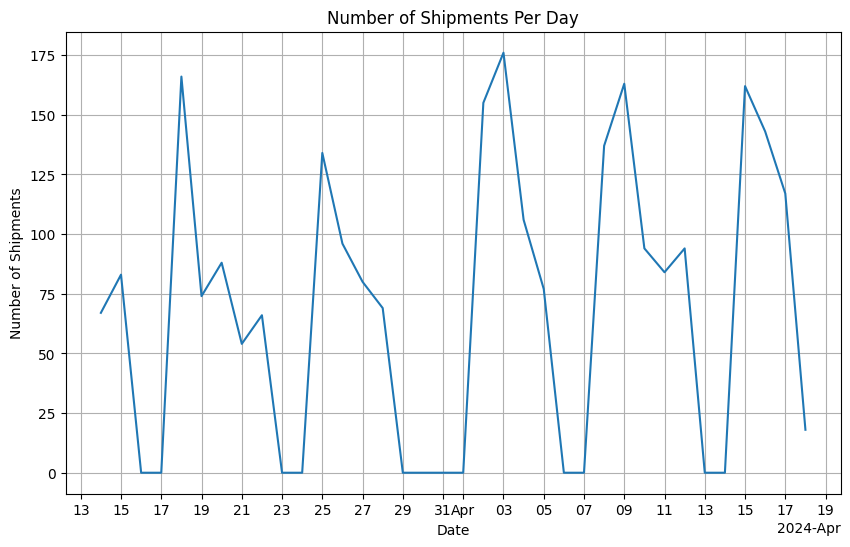
\includegraphics[width=140mm]{img/chap08/shipment_per_day.png}
\caption{Number of shipments per day}
\label{img08:plot:shipment_per_day}
\end{figure}
Integration has been largely seamless. However, during the testing phase, we refined the database queries used to retrieve new shipments several times to meet previously unidentified requirements.
Many of these adjustments stemmed from the need to handle shipments that did not have an associated invoice and only had reference to a packing list.

Furthermore, to provide insight into the workflow of operators and identify peak operational times, we analysed the distribution of shipments sent to the platform within 30-minute intervals during a typical working day.
As illustrated in Figure \ref{img08:plot:shipment_distribution} below, the creation of shipments peaks around lunchtime, aligning closely with the pickup schedule of the shipping carrier between 13:30 and 14:30.
With this data we can additionally optimise the scheduled tasks used for data exchange between SAP and our platform.
\begin{figure}[H]\centering
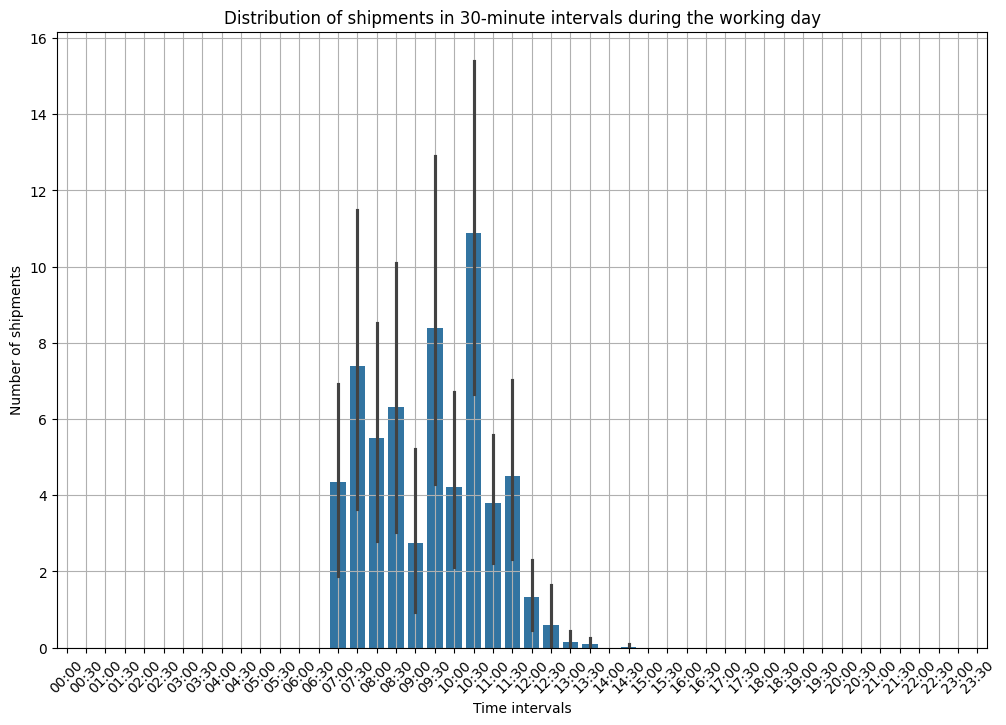
\includegraphics[width=140mm]{img/chap08/shipments_time_intervals.png}
\caption{Distribution of shipments creation in 30-minutes intervals during the work day}
\label{img08:plot:shipment_distribution}
\end{figure}

\subsection{Connecting with shipping carriers}
\label{subsec:connecting-with-shipping-carriers}
Establishing a connection to all three implemented shipping carriers - Packeta, PPL, and Česká Pošta was a smooth process without any issues.
Connecting packeta was straightforward; it involved simply copying the \texttt{API-Key} from Packeta's online administration interface.
This password is all that was required to authenticate and interact with Packeta's API, making the integration process very simple and fast.
For PPL, the credentials needed were a \texttt{ClientID} and a \texttt{Client Secret}, which had to be obtained directly from PPL's support team.
Although this required waiting for the support team to provide the necessary credentials, the overall process went smoothly once the credentials were received.
Integration with Česká Pošta was slightly more involved.
Initially, it required contacting the sales representative of Česká Pošta to ensure that the proper permissions to generate access keys were established in the Česká Pošta client administration portal.
After these permissions were in place, generating the \texttt{API Token} and obtaining \texttt{Secret} was straightforward.
However, additional details such as the postal code of the post office, the customer's ID, and the contract number needed to be specified; these were promptly provided by the sales representative.

With all necessary credentials and configurations set, each carrier's integration was completed and saved under the respective project in platform.
Integration of these carriers represents a critical step in the platform, allowing data transmission between the platform and the shipping carrier.

\subsection{Training and operational challenges}
\label{subsec:training-operational-challenges}
Training the staff, so-called operators, to use the platform was relatively straightforward, thanks to the simplicity principle of the platform design.
The primary interface feature is a main table where operators select rows and execute predefined actions with a single button click.
This simplicity in design minimized the learning curve and helped quick adoption.
Given the fact, that operators use desktop computers with a mouse and keyboard, there were no issues with layout responsibility or accessibility of the dashboard.
Platform's data filtering and manipulation functionalities were also intuitive for the staff.
Most operators already had basic knowledge of software like Excel and were familiar with the SAP Business One user interface, making adoption easier.
Despite the ease of training, there were operational challenges during the initial phases of the deployment.
Adjustments had to made within the shipments table, such as highlighting "today's" orders, setting a row colour for different shipment statuses.
Given that the Packeta API is not among the fastest, which was mostly shown when generating package labels, the implementation of a simple loading bar was necessary.
This loading bar was displayed to the user immediately after clicking the button, completely disabling it.
Several changes were also made to the shipment detail user interface, where some fields were rearranged and added, as well as fixing a bug that made it impossible to edit the pickup point.

From the user perspective, the branded tracking page presents the status of the parcels and basic shipment data.
However, users also have the option to go to the official shipping carrier tracking page.
But the question is do they use it?
We have implemented anonymous event-based user tracking.
\begin{figure}[H]\centering
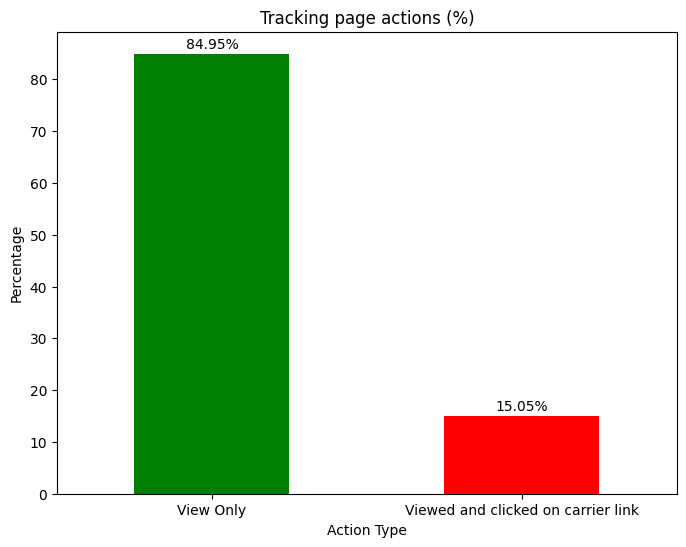
\includegraphics[width=100mm]{img/chap08/tracking_page_events.png}
\caption{Tracking page actions}
\label{img08:plot:tracking_page_actions}
\end{figure}
And, as we can see from the data on Figure \ref{img08:plot:tracking_page_actions}, the significant portion of users is satisfied with what they see on our tracking page and do not need to continue to the carrier's official tracking page at all.
Another interesting thing that arises from tracking page events data is the distribution of device, or to be more precise, screen type.
We have decided to track three device types:
\begin{itemize}
    \item \texttt{desktop:} Everything over approximately 992 px.
    \item \texttt{table:} Everything over approximately 768 px.
    \item \texttt{mobile:} The rest.
\end{itemize}
Although we expected that most of the users will open the tracking page from their phone, the data in Figure \ref{img08:plot:tracking_page_device_type} show something different.
Phone users are certainly not insignificant, but the desktop leads the way.
\begin{figure}[H]\centering
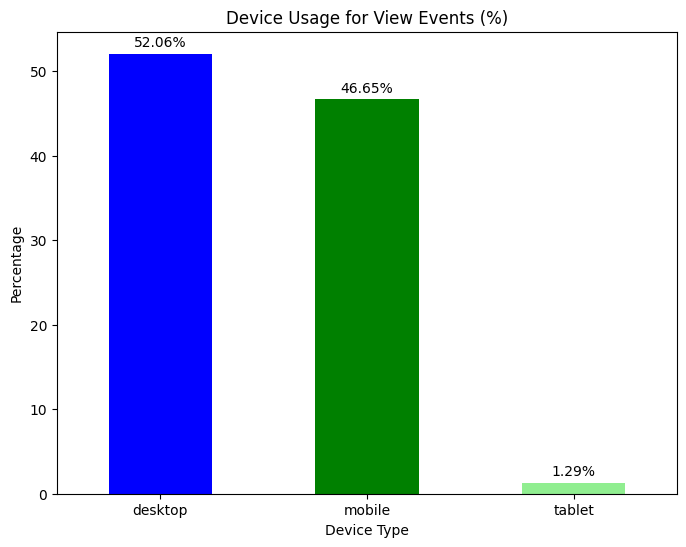
\includegraphics[width=100mm]{img/chap08/tracking_page_devices.png}
\caption{Device usage for view events (\%)}
\label{img08:plot:tracking_page_device_type}
\end{figure}

\subsection{Operational performance and business impact}
\label{subsec:operational-performance-business-impact}
The operational performance of the platform has been robust, supported by the detailed \gls{aws-cloudwatch} monitoring.
Analysis of the Lambda invocation duration in Figure \ref{img08:plot:lambda_handler_durations} reveals that the average response time during peak periods can reach up to 4 seconds on average, which is still within the Lambda tolerance.
So, just raising the timeout should be enough for these special cases described below.
However, normally, this number is well below 250 miliseconds.
\begin{figure}[H]\centering
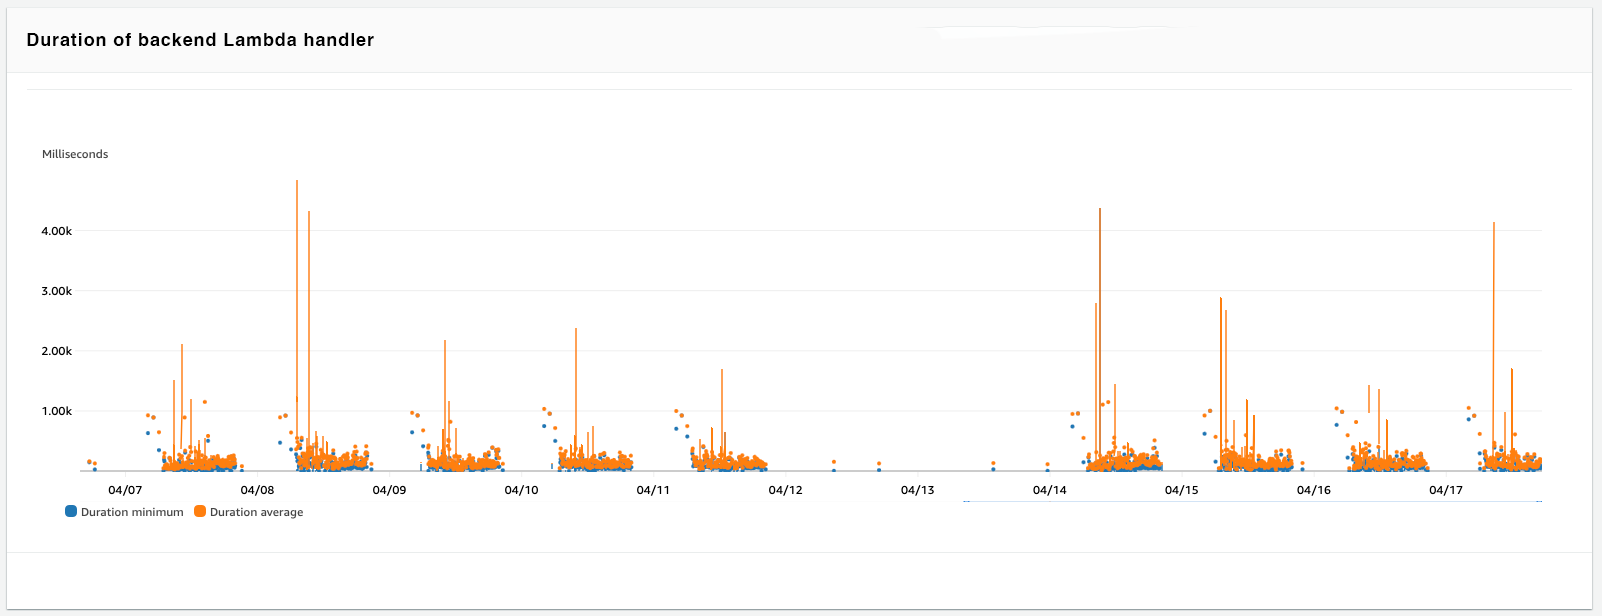
\includegraphics[width=140mm]{img/chap08/lambda_handler_durations.png}
\caption{Duration of backend Lambda handler}
\label{img08:plot:lambda_handler_durations}
\end{figure}
The high average is typically associated with requests for shipping labels or operations involving the Packeta API, which tends to have slower response times due to the need to await responses with the Lambda function.
Furthermore, the error and success rates monitored through \gls{aws-cloudwatch} in Figure \ref{img08:plot:lambda_handler_errors} indicate a very high availability of the system. The metrics show a minimal error rate, which underscores the robustness and reliability of the backend Lambda handler. This high success rate ensures that the system remains dependable under various operational conditions, providing a stable and efficient service to users.
\begin{figure}[H]\centering
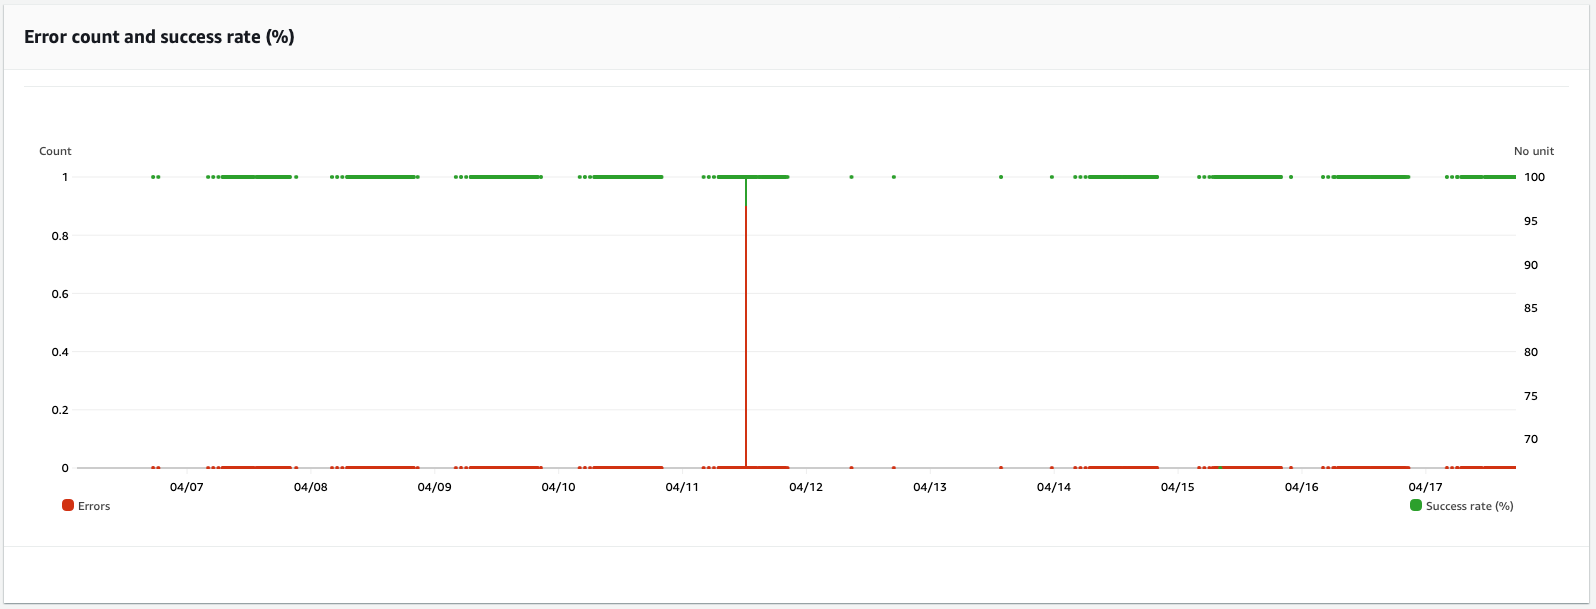
\includegraphics[width=140mm]{img/chap08/lambda_handler_errors.png}
\caption{Error count and success rate (\%) of backend Lambda handler}
\label{img08:plot:lambda_handler_errors}
\end{figure}

The business impact of the platform has been largely positive.
Transitioning from an older, difficult to maintain system to this modern platform, has moved the company's logistic operations into a good direction.
The previous system, while functional, suffered from poor architecture and limited accessibility, restricting usage to only a network within the company.
Not only that, but operators could not anyhow edit the data in the old system. 
Meaning that they had to do all minor changes in the SAP Business One, making the whole job much more difficult. 
In contrast, the new platform offers flexibility and remote accessibility, allowing staff to interact with the system from any location using mobile devices.

This improvement in accessibility and user experience is complemented by the extensibility of the platform. 
The architecture of the new system is designed to facilitate integration with different carriers and allow for very straightforward integrations with new carriers and updates within existing APIs. 
This capability is particularly valuable in today's dynamic business environment, where shipping conditions and costs can change frequently, making it unsuitable for the business.
The platform design allows the business to quickly adapt to these changes by enabling a seamless transition to different carriers as needed, as long as the carrier implementation is present.
Or, the business can request the implementation of a new carrier, which generally should be a complex problem given the platform carrier integration design. 
This adaptability not only provides operational flexibility, but also gives the company a competitive advantage in logistics management and enhances its ability to respond effectively to market changes and customer needs.


\subsection{Achievement of project goals}
\label{subsec:achievement-project-goals}
%  how were all goals fullfied and tested
% the goals are:
% G1 Streamline logistics operations: Develop a platform that simplifies the process of dispatching orders to shipping carriers, automating data ex- change, and minimizing need for manual intervention.
% G2 Modern cloud based multi-tenant solution: Create application with multi-tenant architecture allowing it to be used by multiple companies de- ployed to the cloud with automated integration and deployment.
% G3 Create branded shipping customer experience: Introduce a new mar- keting communication platform using the data collected from the shipping carrier that allowed each company to specify custom branding for the parcel tracking page and parcel status notification emails.

% G4  Integration with existing systems: Develop a solution that can be easily integrated with existing businesses’ system.

% G5: Validate in a real-world setting with SAP Business One integra- tion: Test the platform in a live e-Commerce environment, handling a significant volume of orders in daily operations.


% for a goal about dashboard - dashboard ís used for all data sending processes, label generation and even manual intervention into the shipment data

At the beginning of the development of this platform, we set five main goals, as outlined in \hyperref[subsec:project-goals]{Project goals}. 
These objectives were aiming to improve the expedition process of the eCommerce companies by automating interactions with shipping carriers, enhancing customer engagement through branded tracking page, and ensuring simple integration with existing systems. 
Here, we evaluate and reflect on how these goals were fulfilled through the deployment and real-world application of the platform.

\begin{enumerate}[label=\bfseries G\arabic*:,leftmargin=*]
    \item \textbf{Streamline logistics operations:} The platform has effectively simplified the process of dispatching orders to shipping carriers by automating data exchanges and minimizing manual intervention. 
    This was achieved through a user-friendly dashboard that facilitates all data sending processes and label generation, thus streamlining logistics operations.
    Refer to Figure \ref{img08:fig:shipment_list} for a view of the dashboard shipment list with filtering, Figure \ref{img08:fig:shipment_edit} for the shipment edit interface and Figure \ref{img08:fig:shipment_view} for the detailed shipment view.
    Please note that the data shown in the examples are mocked, and not actual customer data.
    \begin{figure}[H]\centering
    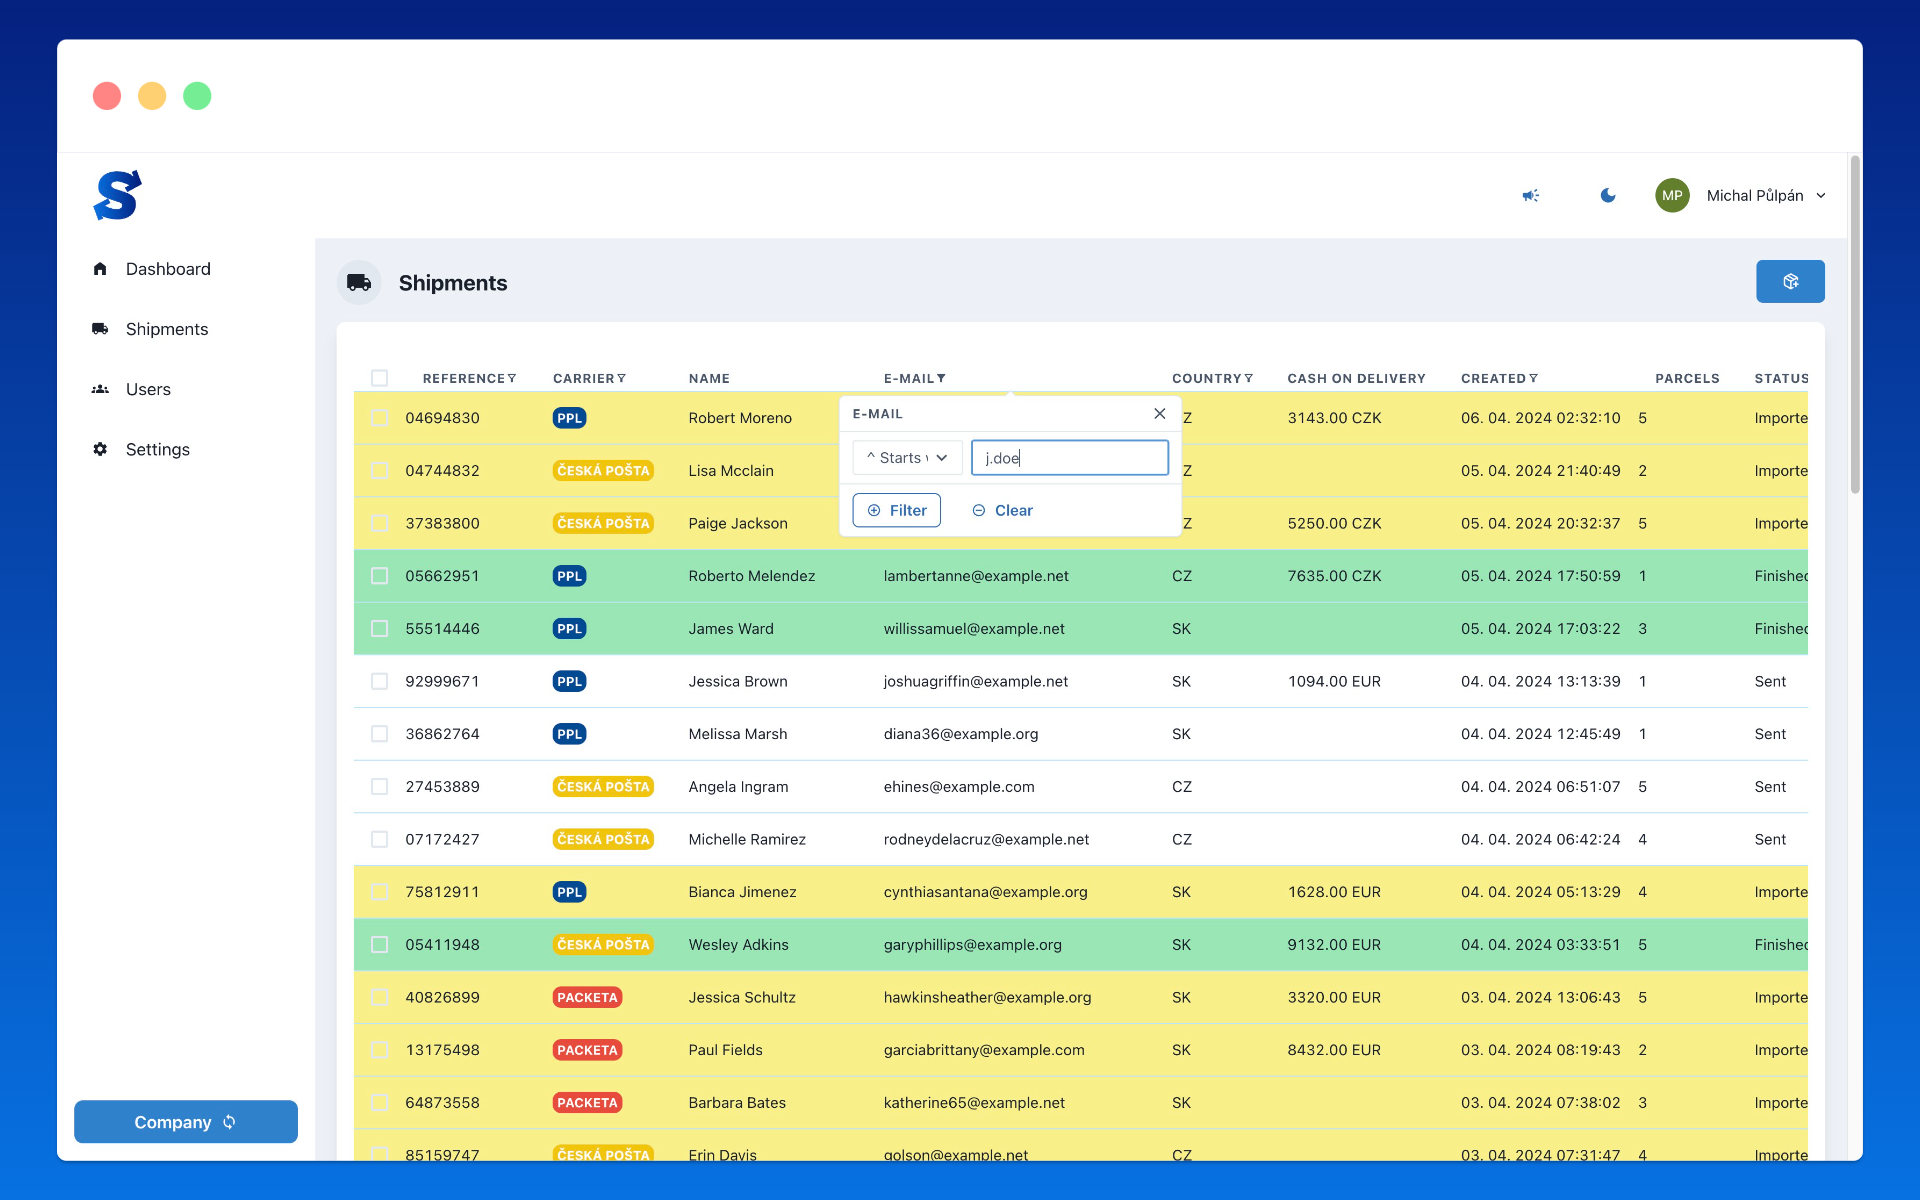
\includegraphics[width=140mm]{img/chap08/gui_shipment_list.png}
    \caption{Dashboard shipment list with filtering}
    \label{img08:fig:shipment_list}
    \end{figure}
    \begin{figure}[H]\centering
    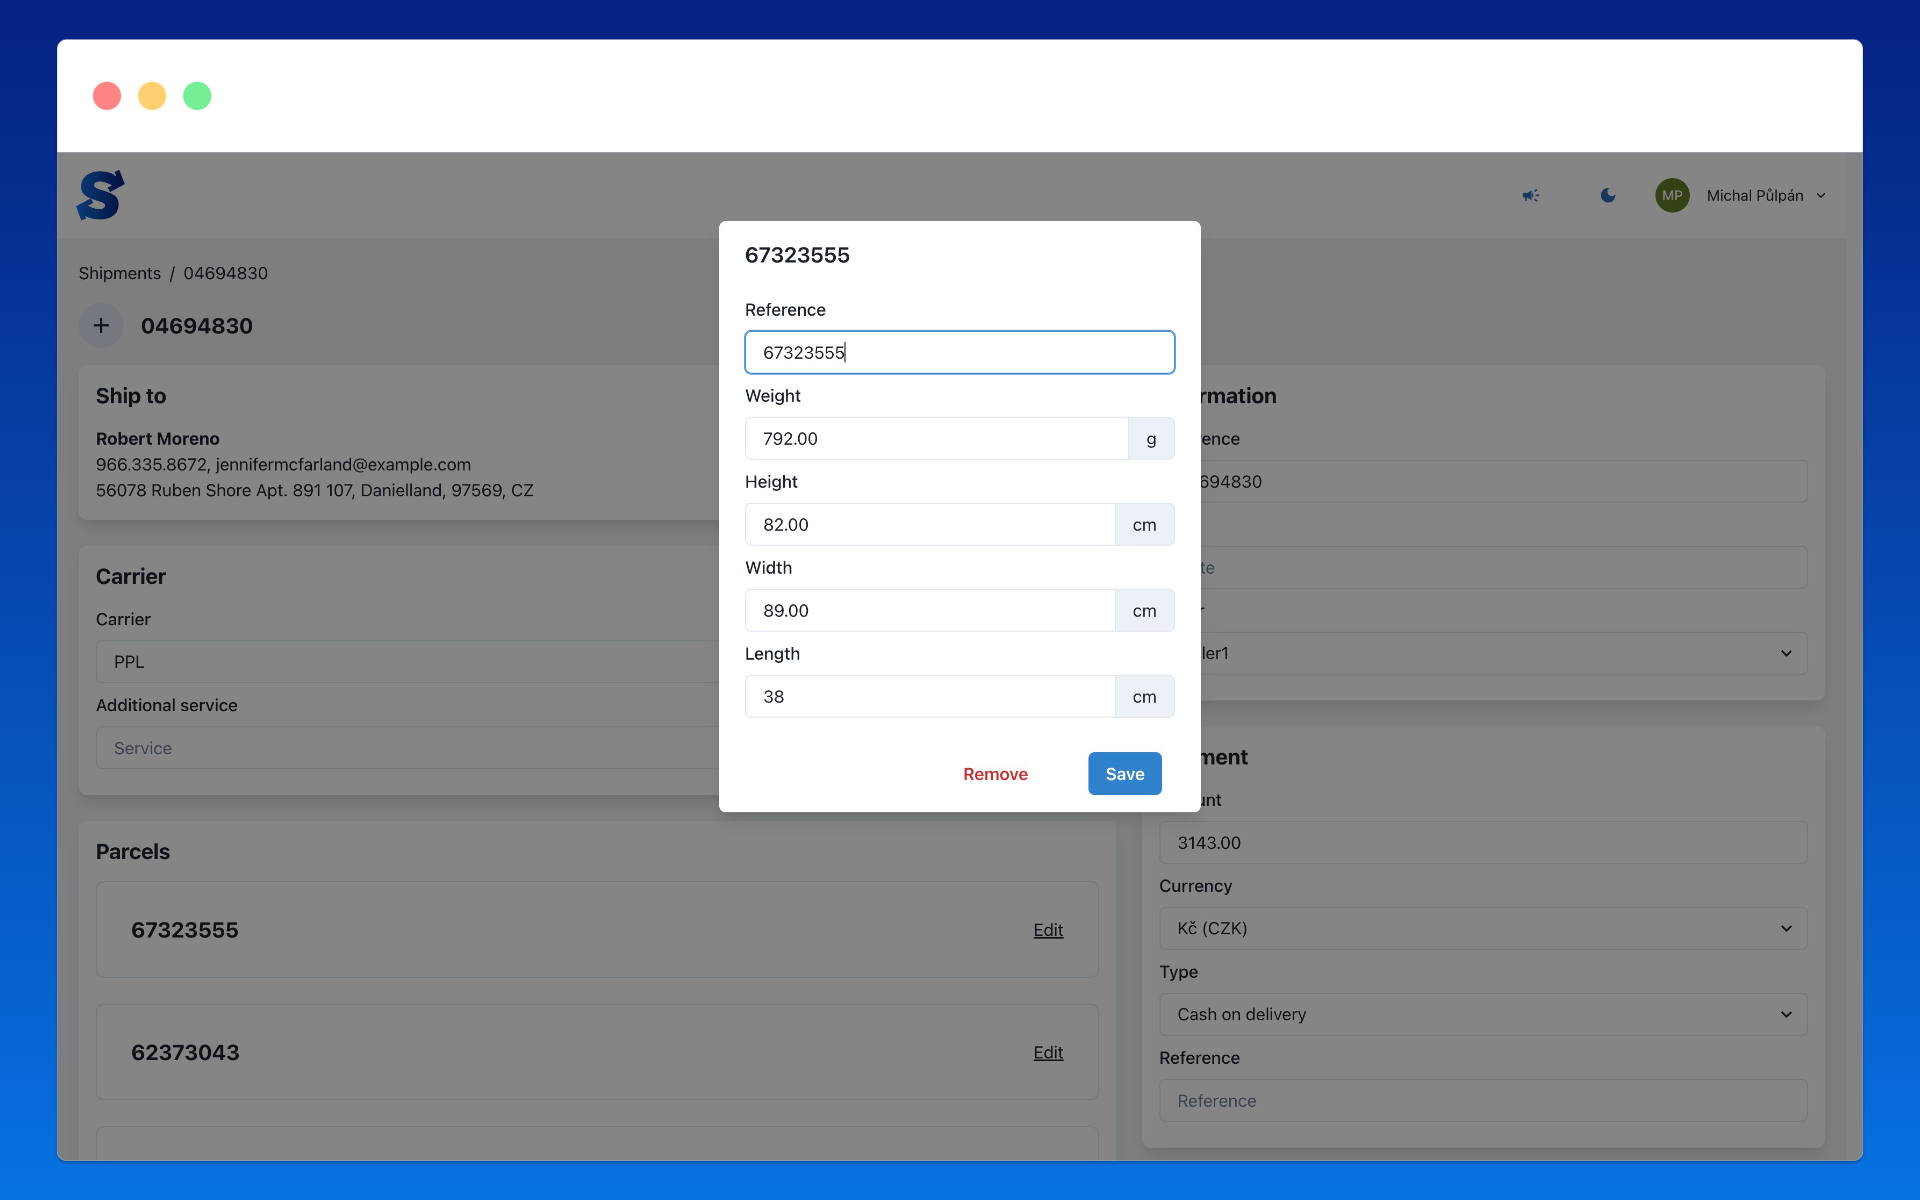
\includegraphics[width=140mm]{img/chap08/gui_shipment_detail.png}
    \caption{Dashboard shipment edit mode}
    \label{img08:fig:shipment_edit}
    \end{figure}
    \begin{figure}[H]\centering
    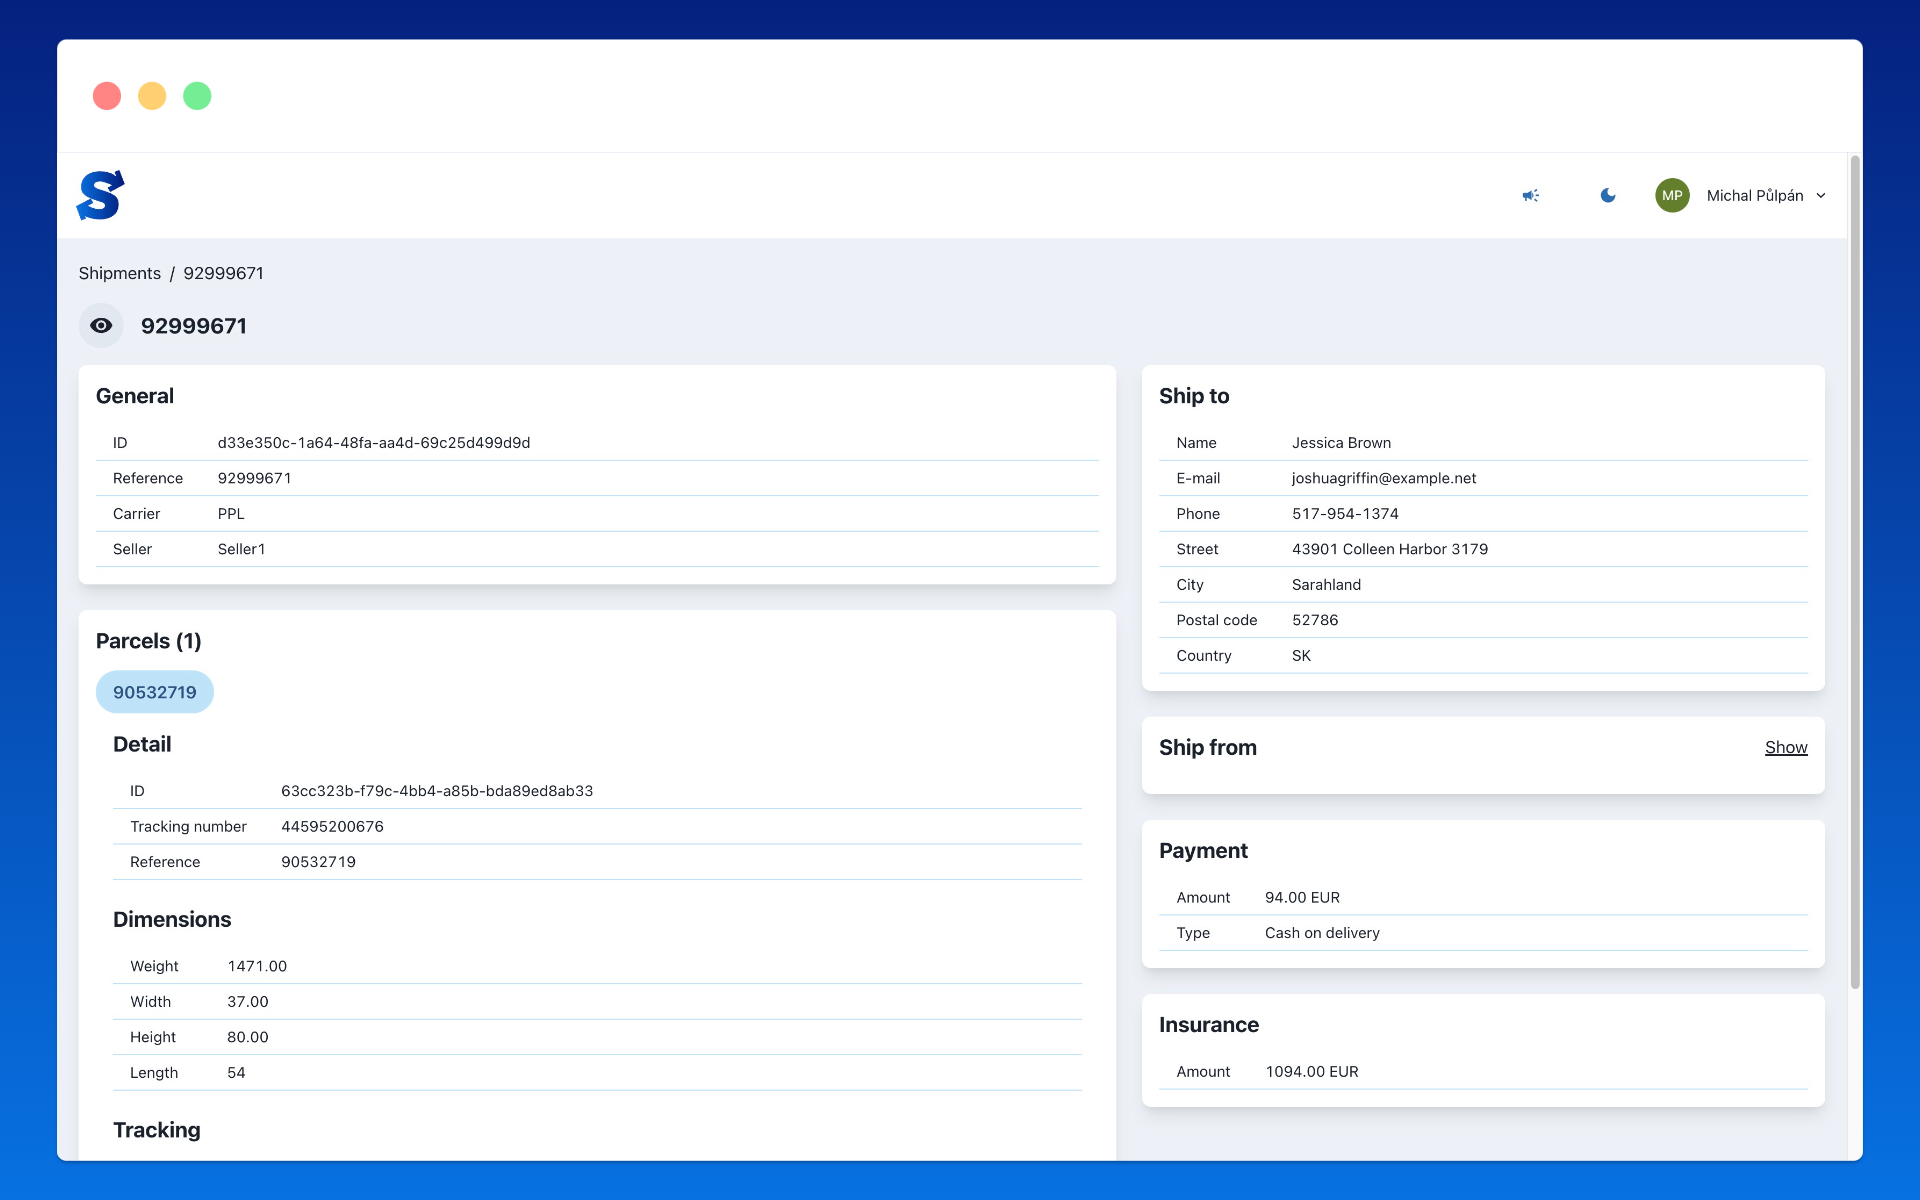
\includegraphics[width=140mm]{img/chap08/gui_shipment_view.png}
    \caption{Dashboard shipment view mode (after being sent)}
    \label{img08:fig:shipment_view}
    \end{figure}
    
    \item \textbf{Modern cloud based multi-tenant solution:} Developed with a multi-tenant architecture, the platform supports multiple companies simultaneously.
    The platform uses Amazon Web Services as a deployment infrastructure. 
    This structure with the use of a serverless deployment ensures that the platform can easily adapt to growing business needs while maintaining performance and data security.
    % TODO: přidat seznam projektů? nebo seznam uživatelů?
    
    \item \textbf{Create branded shipping customer experience:} The platform enhances the post-purchase experience by allowing businesses to customise the branding of parcel tracking pages and email notifications.
    Customisation is done through an intuitive configuration interface within the dashboard.
    This covers standard operational processes into valuable marketing opportunities, creating a new marketing channel while increasing customer engagement and strengthening brand identity.
    Figure \ref{img08:fig:tracking_config} shows the configuration page where businesses can set the branding for their tracking pages and email notifications. Figure \ref{img08:fig:email_notification} shows an example of an email notification for a package sent to an Austrian customer, illustrating how multiple branding layouts can be managed in a single account.
    \begin{figure}[H]\centering
    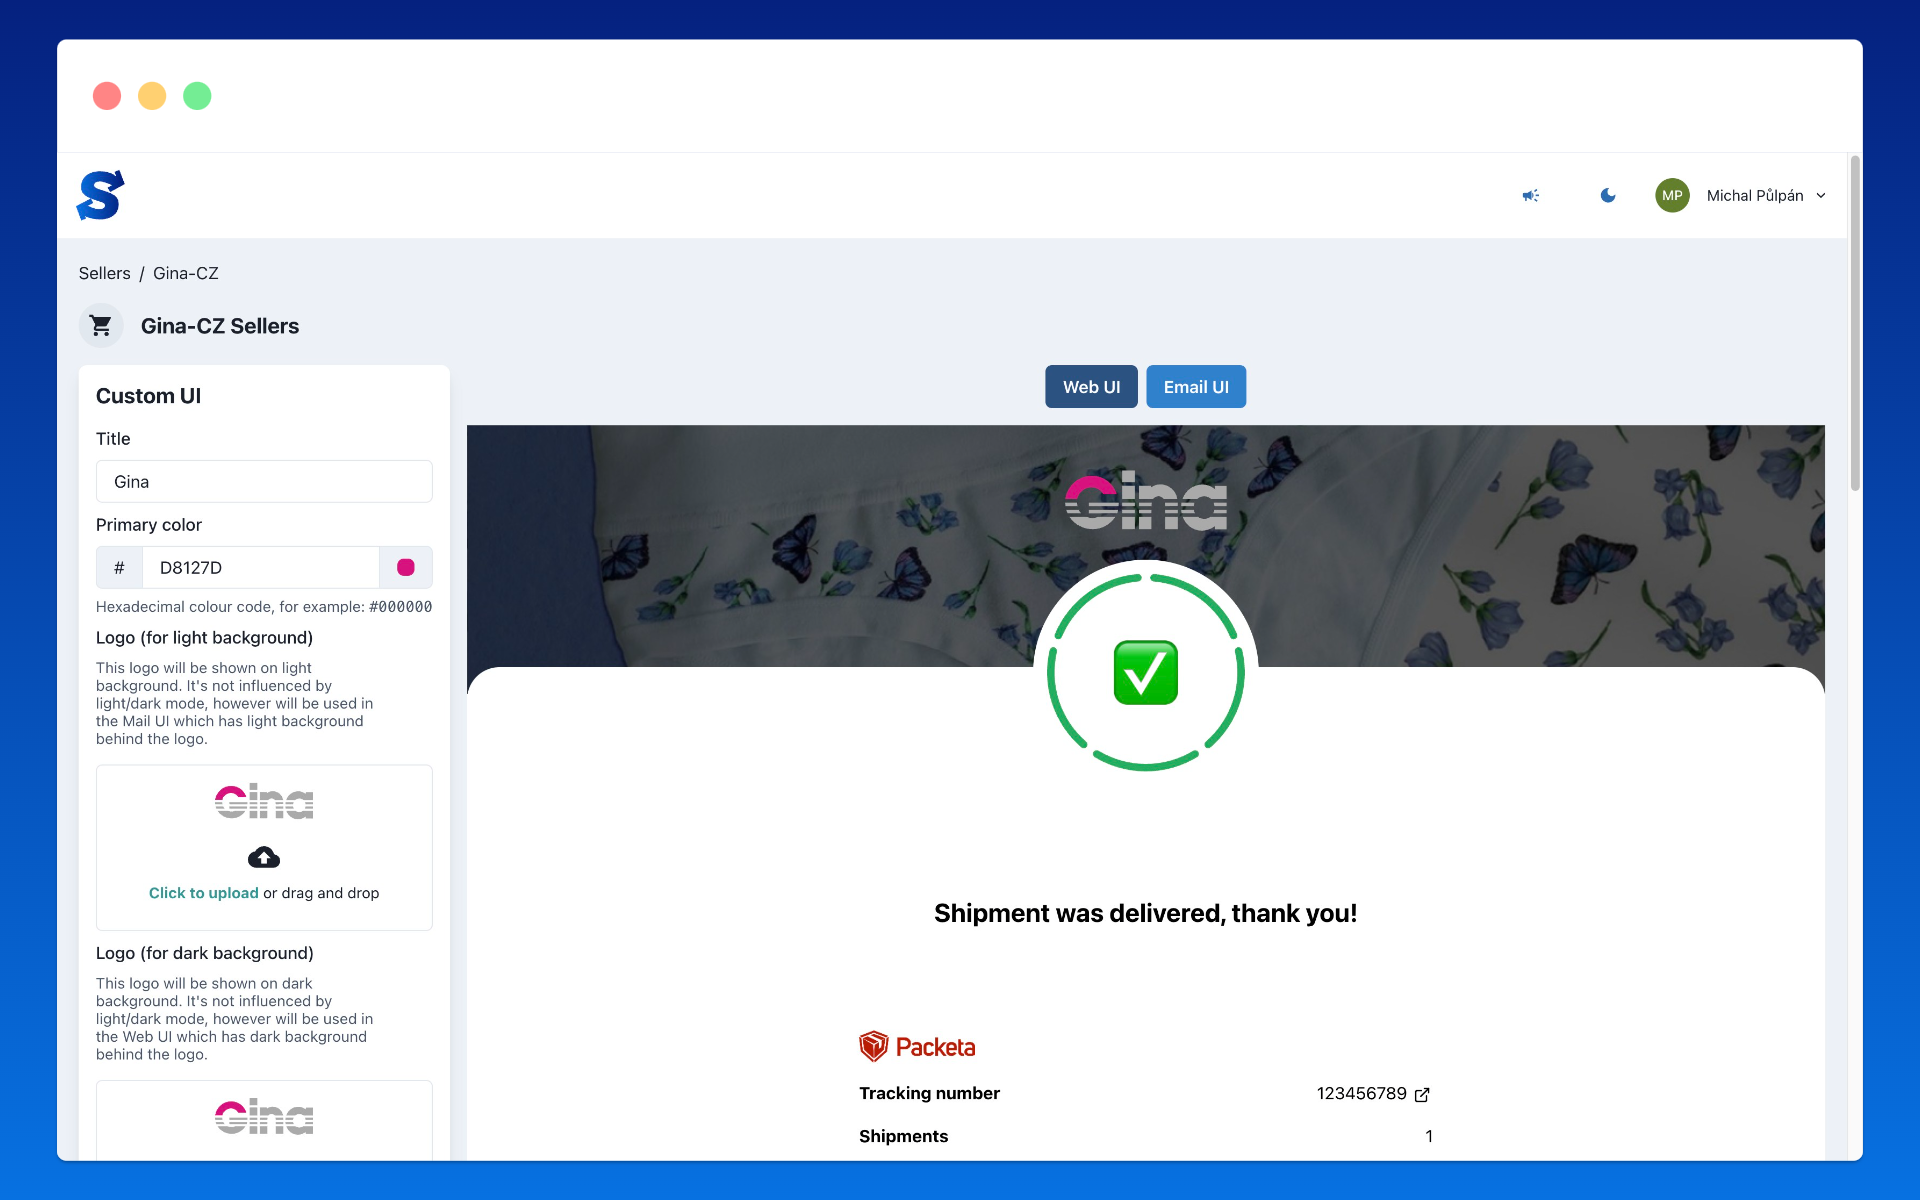
\includegraphics[width=140mm]{img/chap08/gui_branding_cinfiguration.png}
    \caption{Dashboard tracking page/email notification branding configuration page}
    \label{img08:fig:tracking_config}
    \end{figure}
    \begin{figure}[H]\centering
    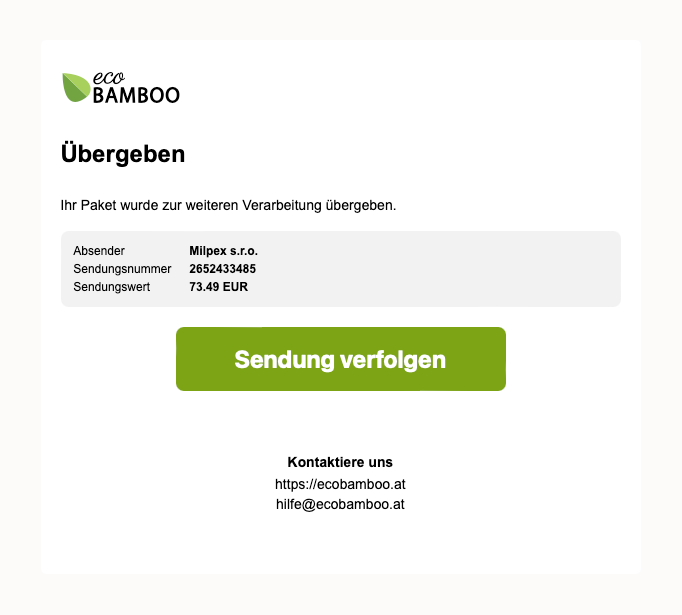
\includegraphics[width=140mm]{img/chap08/email_notification.png}
    \caption{Email notification of shipped parcel for Austrian customer}
    \label{img08:fig:email_notification}
    \end{figure}
    
    \item \textbf{Integration with existing systems:} Seamless integration with existing business systems, particularly SAP Business One, was an important aspect of the platform.
    The platform facilitates this through public API that offers the same services provided by the dashboard, including creating and modifying shipments, generating labels, retrieving filtered shipments, and much more.
    This allows for integration flexibility and the ability to automate processes externally from the platform interface. Figure \ref{img08:fig:user_documentation} shows the on-line user documentation interface that helps users navigate and utilise the platform features effectively. Figure \ref{img08:fig:swagger_documentation} displays the Swagger public API documentation, which is instrumental for developers looking to seamlessly integrate their systems with the platform.
    % Přidat screenshot z docs?
    \begin{figure}[H]\centering
    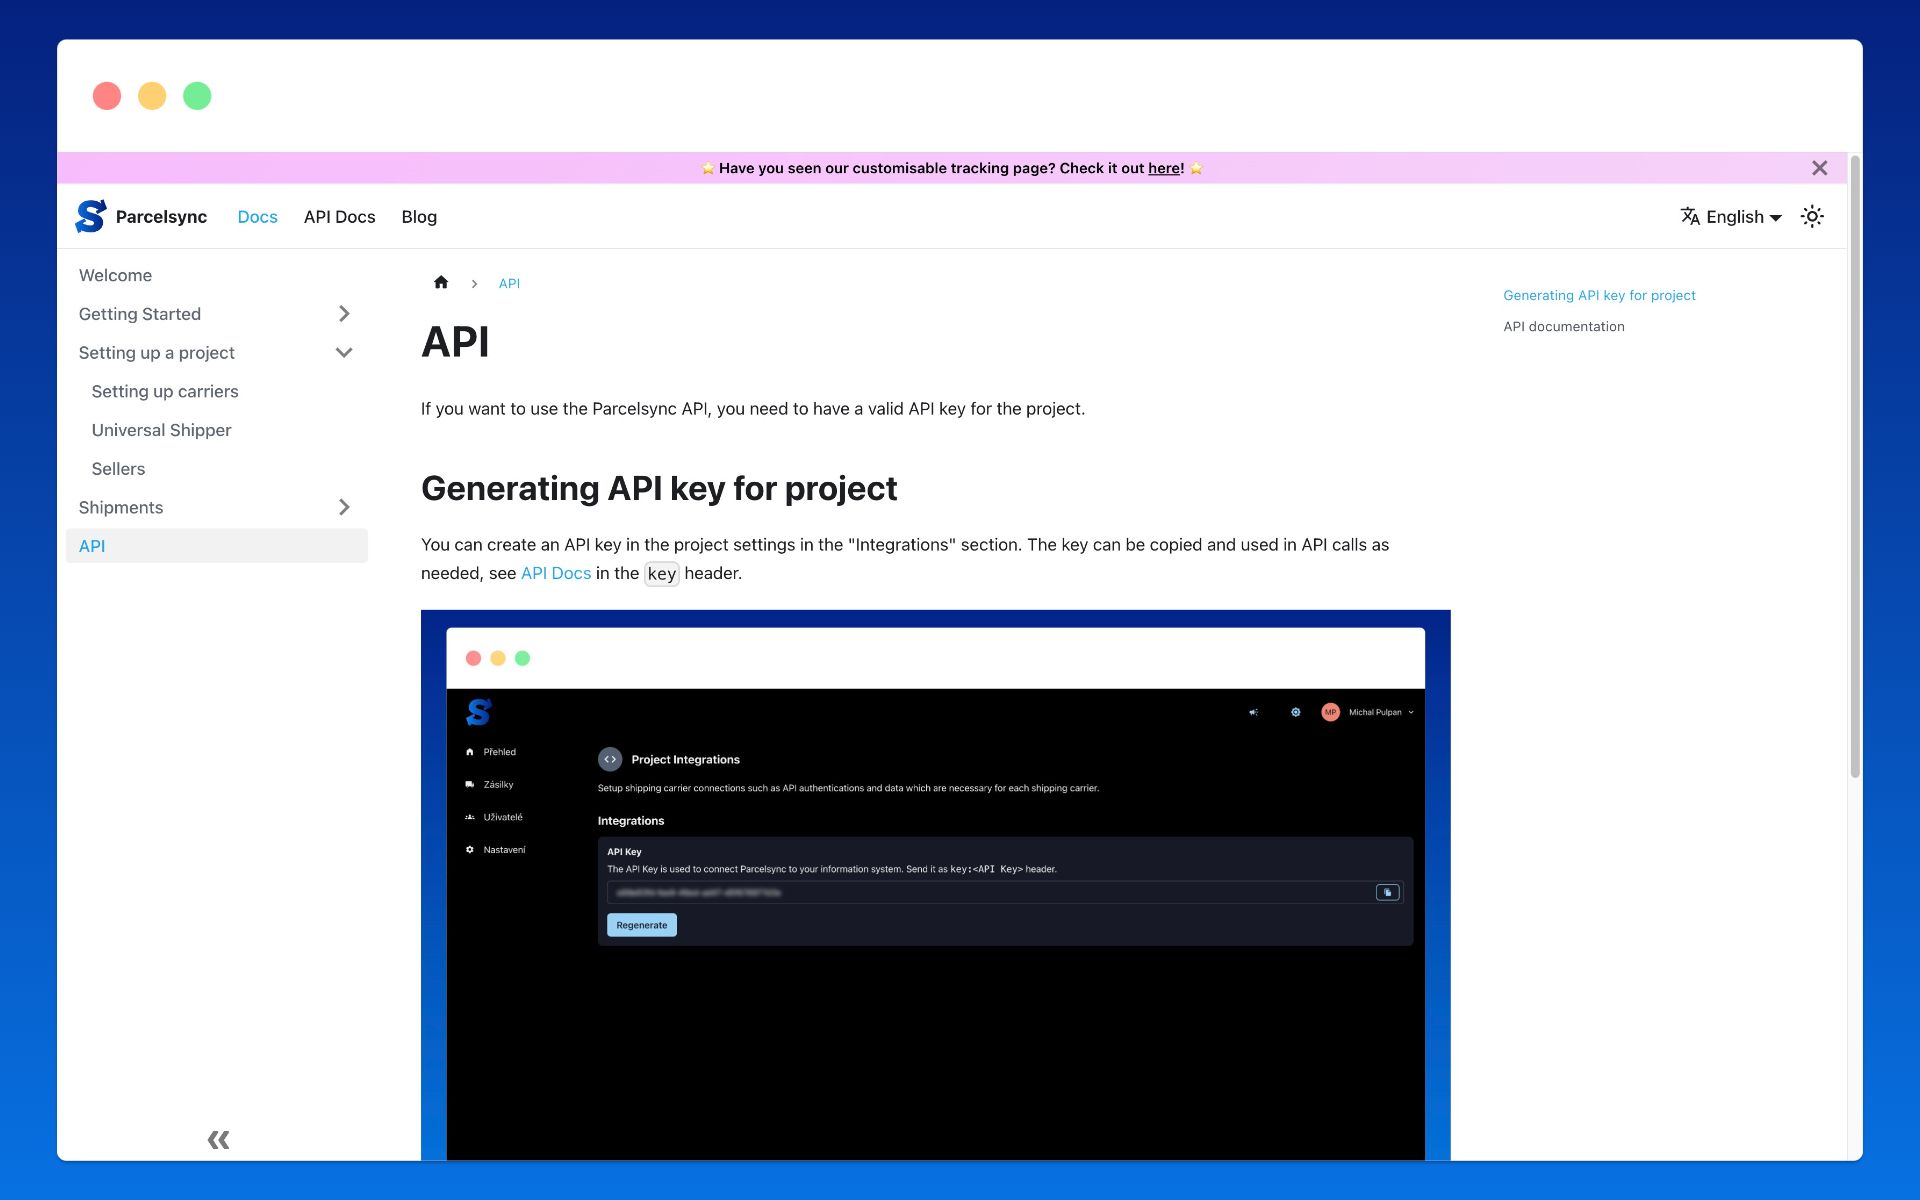
\includegraphics[width=140mm]{img/chap08/user_documentation.png}
    \caption{Online user documentation interface}
    \label{img08:fig:user_documentation}
    \end{figure}
    \begin{figure}[H]\centering
    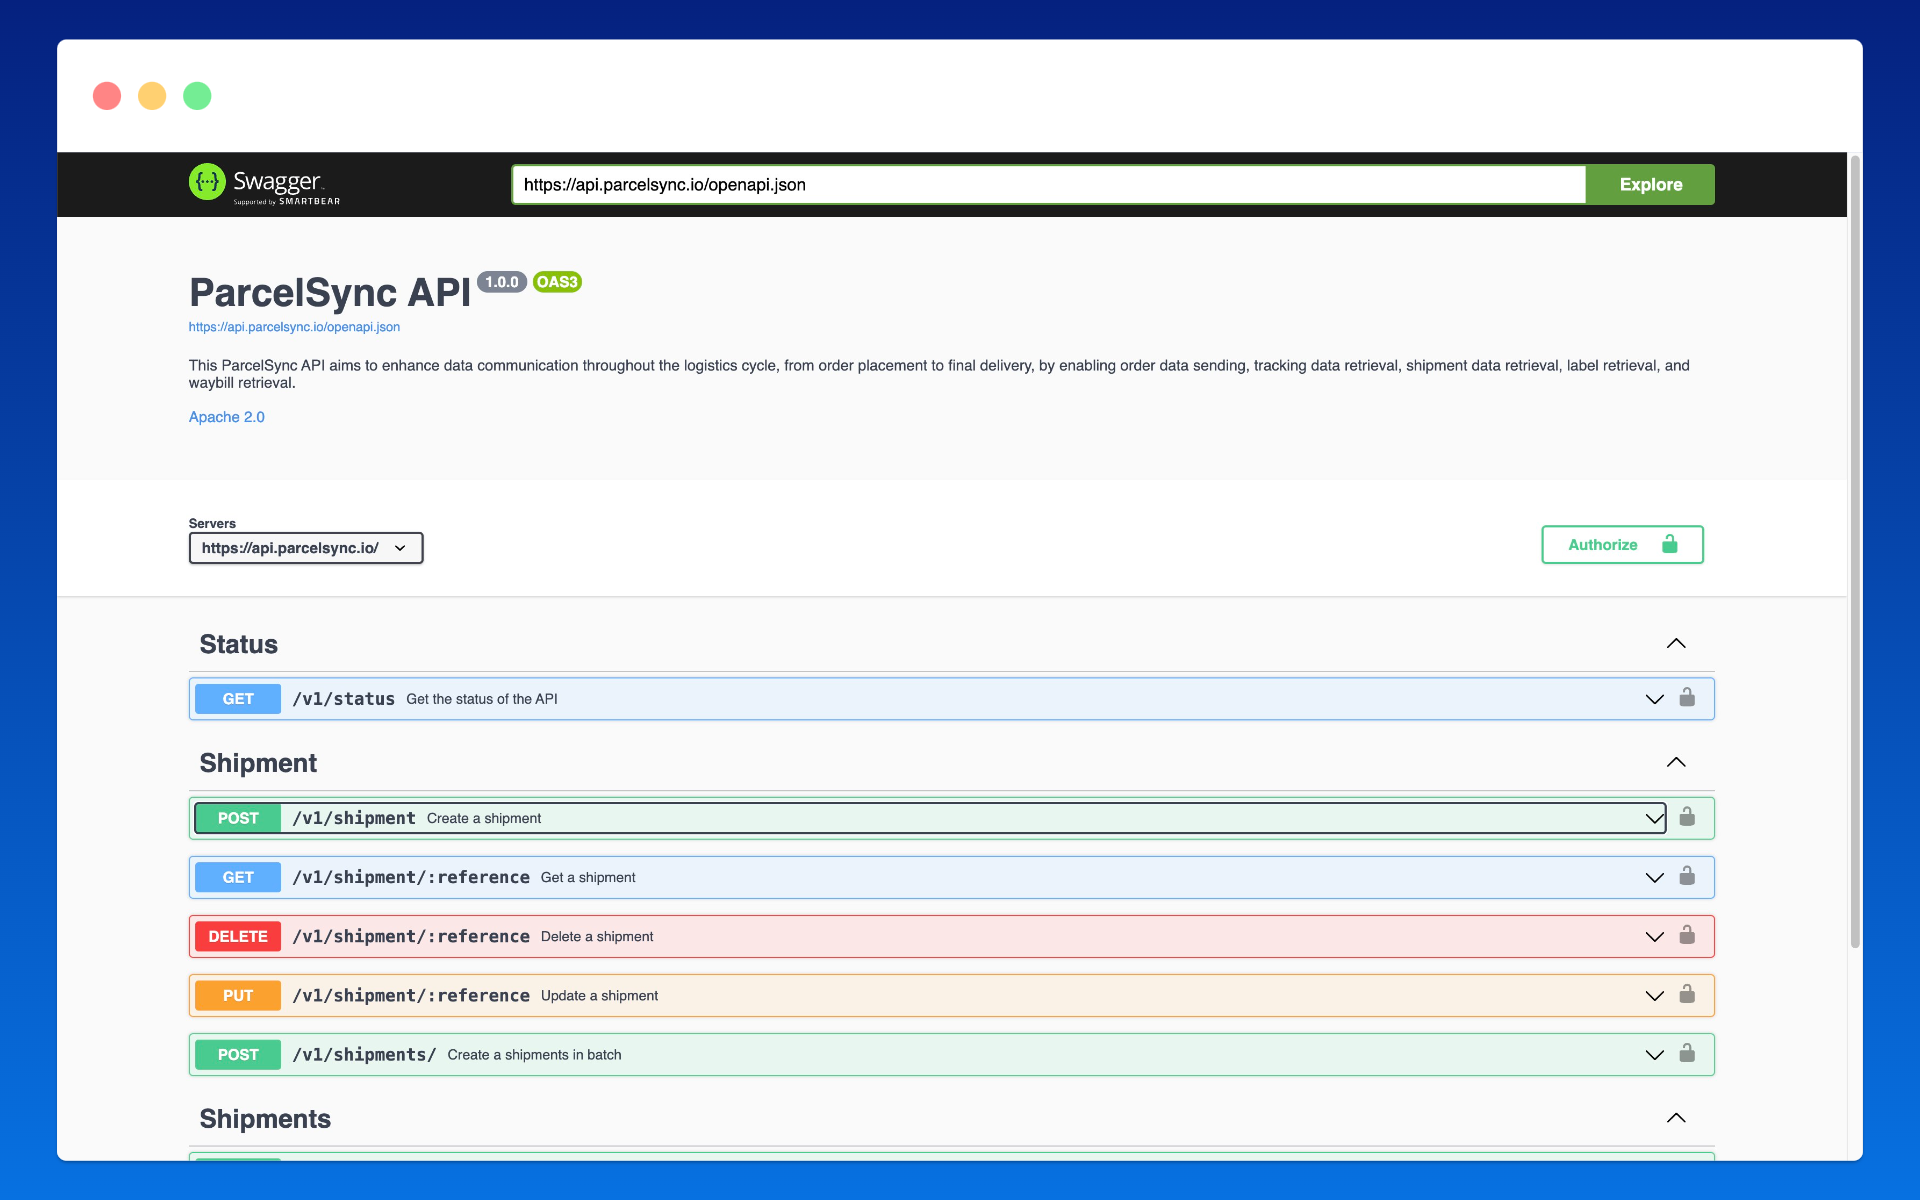
\includegraphics[width=140mm]{img/chap08/swagger_documentation.png}
    \caption{Swagger public API documentation}
    \label{img08:fig:swagger_documentation}
    \end{figure}
    
    \item \textbf{Validate in a real-world setting with SAP Business One integration:} The effectiveness of the platform has been thoroughly tested in a real eCommerce environment, which manages more than 100 shipments per day. 
    This real-world testing, integrated with SAP Business One, demonstrated the robustness and operational reliability of the platform.
    Figure \ref{img08:plot:recipients_distribution} showing the spatial distribution of the recipients of the shipment during the first month of use of the production.
    \begin{figure}[H]\centering
    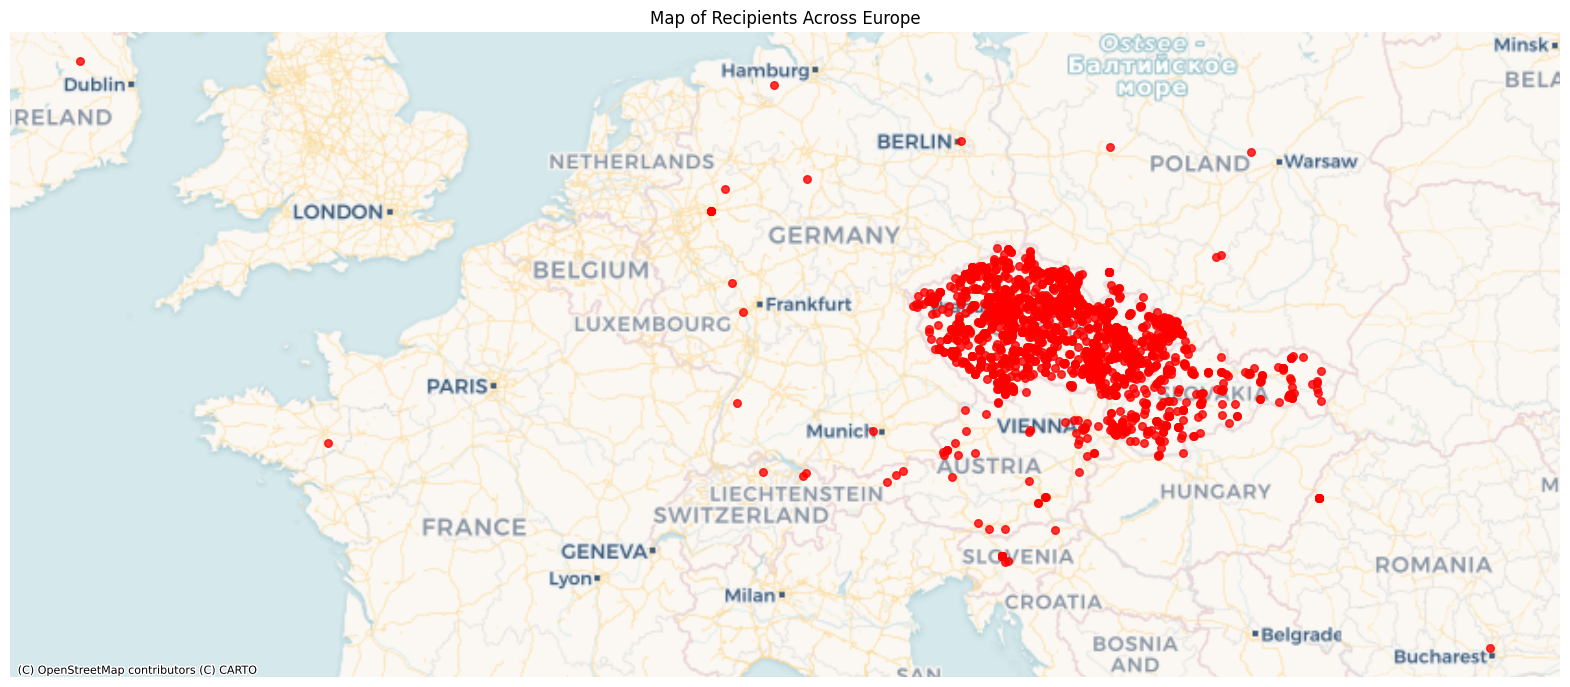
\includegraphics[width=140mm]{img/chap08/recipients_europe.png}
    \caption{Distribution of recipients within Europe}
    \label{img08:plot:recipients_distribution}
    \end{figure}
\end{enumerate}

This chapter has evaluated the operational efficacy and integration of the \ac{SaaS} platform within a real-world business environment.
During this evaluation, the platform has been shown to meet operational requirements by simplifying logistics processes, enhancing customer interaction through branded experiences, and integrating with existing business systems. 
By achieving these objectives, the platform not only fulfils the set project goals but also establishes a foundation for future expansions and optimisations in eCommerce logistics. 
The platform provides a clear direction for continued innovation and improvement, ensuring that the platform can continue to deliver business value as market conditions evolve.

%\section{User Interface Overview}

%\subsection{Shipment Management Interface}
% with mobile and responsive design

%\subsection{Project management}
% users, settings, carrier integrations

%\subsection{Brand customization}

%\subsection{Tracking page and email notifications}
% with mobile and responsive design

